% ! Tex program = xelatex
\documentclass{article}
% \PassOptionsToPackage{quiet}{fontspec}% (or try silent)
% 中文
% \usepackage[UTF8]{ctex}

% For more choices
% %! Tex program = xelatex
% \documentclass{article}
%中文
%\usepackage[UTF8]{ctex}
%数学公式
\usepackage{amsmath,amssymb}
%\usepackage{ntheorem}
% \usepackage[framemethod=TikZ]{mdframed}
\usepackage{amsthm}
%边界
\usepackage[letterpaper,top=3cm,bottom=3cm,left=2cm,right=2cm,marginparwidth=1.75cm]{geometry}%table package
%Table
\usepackage{multirow,booktabs}
\usepackage{makecell}
%字体颜色
\usepackage{color}
\usepackage[dvipsnames]{xcolor}  % 更全的色系
%代码
\usepackage[OT1]{fontenc}
% MATLAB 代码风格
% \usepackage[framed,numbered,autolinebreaks,useliterate]{/Users/anye_zhenhaoyu/Desktop/Latex/mcode}
\usepackage{listings}
\usepackage{algorithm}
\usepackage{algorithmic}
\usepackage{pythonhighlight} % Python
%插图
\usepackage{graphicx}
%改变item格式
\usepackage{enumerate}
%物理
\usepackage{physics}
%extra arrows
\usepackage{extarrows}
% caption(居中指令)
\usepackage[justification=centering]{caption}
% \usepackage{caption}
% htpb
\usepackage{stfloats}
% pdf 拼接
\usepackage{pdfpages}
% 超链接url
\usepackage{url}
% \usepackage{tikz}
\usepackage{pgfplots}
\pgfplotsset{compat=newest}
\usepackage[colorlinks=true, allcolors=blue]{hyperref}
\usepackage{setspace}

% --------------definations-------------- %
\def\*#1{\boldsymbol{#1}}
\def\+#1{\mathcal{#1}} 
\def\-#1{\bar{#1}}
% Domains
\def\RR{\mathbb{R}}
\def\CC{\mathbb{C}}
\def\NN{\mathbb{N}}
\def\ZZ{\mathbb{Z}}
% Newcommand
\newcommand{\inner}[2]{\langle #1,#2\rangle} 
\newcommand{\numP}{\#\mathbf{P}} 
\renewcommand{\P}{\mathbf{P}}
\newcommand{\Var}[2][]{\mathbf{Var}_{#1}\left[#2\right]}
\newcommand{\E}[2][]{\mathbf{E}_{#1}\left[#2\right]}
\renewcommand{\emptyset}{\varnothing}
\newcommand{\ol}{\overline}
\newcommand{\argmin}{\mathop{\arg\min}}
\newcommand{\argmax}{\mathop{\arg\max}}
\renewcommand{\abs}[1]{\qty|#1|}
\newcommand{\defeq}{\triangleq} % triangle over =
\def\deq{\xlongequal{def}} % 'def' over =
\def\LHS{\text{LHS}}
\def\RHS{\text{RHS}}
\def\angbr#1{\langle#1\rangle} % <x>

\def\Esolve{\textcolor{blue}{Solve: }}
\def\Eproof{\textcolor{blue}{Proof: }}
\def\case#1{\textcolor{blue}{Case \uppercase\expandafter{\romannumeral#1}: }}

\newtheorem{lemma}{Lemma}
\newtheorem{thm}{Theorem}
\newtheorem{defi}{Definition}
\newtheorem{prp}{Proposition}
\newenvironment{md}{\begin{mdframed}}{\end{mdframed}}

\date{\today}
\usepackage{fancyhdr}
\pagestyle{fancy}
\fancyhead[L]{\slshape{Haoyu Zhen}}
\fancyhead[R]{{\today}}

% \begin{document}
% \title{<++>}
\author{Haoyu Zhen}
% \maketitle
\setlength{\parindent}{0pt}
\setstretch{1.2}
% \end{document}


% % theorems
\usepackage{thmtools}
\usepackage{thm-restate}
\usepackage[framemethod=TikZ]{mdframed}
\mdfsetup{skipabove=1em,skipbelow=0em, innertopmargin=12pt, innerbottommargin=8pt}

\theoremstyle{definition}

\declaretheoremstyle[headfont=\bfseries\sffamily, bodyfont=\normalfont,
	mdframed={
		nobreak,
		backgroundcolor=brown!14,
		topline=false,
		rightline=false,
		leftline=true,
		bottomline=false,
		linewidth=2pt,
		linecolor=brown!180,
	}
]{thmbrownbox}

\declaretheoremstyle[headfont=\bfseries\sffamily, bodyfont=\normalfont,
	mdframed={
		nobreak,
		backgroundcolor=Blue!4,
		topline=false,
		rightline=false,
		leftline=true,
		bottomline=false,
		linewidth=2pt,
		linecolor=NavyBlue!120,
	}
]{thmbluebox}

\declaretheoremstyle[headfont=\bfseries\sffamily, bodyfont=\normalfont,
	mdframed={
		nobreak,
		backgroundcolor=Green!5,
		topline=false,
		rightline=false,
		leftline=true,
		bottomline=false,
		linewidth=2pt,
		linecolor=OliveGreen!120,
	}
]{thmgreenbox}

\declaretheoremstyle[headfont=\bfseries\sffamily, bodyfont=\normalfont,
	mdframed={
		nobreak,
		topline=false,
		rightline=false,
		leftline=true,
		bottomline=false,
		linewidth=2pt,
		linecolor=OliveGreen!120,
	}
]{thmgreenline}

\declaretheoremstyle[headfont=\bfseries\sffamily, bodyfont=\normalfont,
	mdframed={
		nobreak,
		topline=false,
		rightline=false,
		leftline=true,
		bottomline=false,
		linewidth=2pt,
		linecolor=NavyBlue!70,
	}
]{thmblueline}

\declaretheorem[numberwithin=section, style=thmbrownbox, name={\color{Brown}Definition}]{defi}
\declaretheorem[numberwithin=section, style=thmgreenbox, name={\color{OliveGreen}Law}]{law}
\declaretheorem[numberwithin=section, style=thmbluebox, name={\color{Blue}Corollary}]{cor}
\declaretheorem[numberwithin=section, style=thmgreenline, name={\color{OliveGreen}Property}]{prt}
\declaretheorem[numberwithin=section, style=thmbluebox, name={\color{Blue}Proposition}]{prp}
\declaretheorem[numberwithin=section, style=thmbluebox, name={\color{Blue}Theorem}]{thm}
\declaretheorem[numberwithin=section, style=thmbluebox, name={\color{Blue}Lemma}]{lemma}
\declaretheorem[numberwithin=section, style=thmbrownbox,  name={\color{Brown}Example}]{eg}
\declaretheorem[numberwithin=section, style=thmgreenline, name={\color{OliveGreen}Remark}]{remark}
\declaretheorem[numbered=no,style=thmblueline, name={\color{NavyBlue!70}Proof},qed=$\square$]{prf}
\numberwithin{equation}{section}


% %! Tex program = xelatex
% \documentclass{article}
%中文
%\usepackage[UTF8]{ctex}
%数学公式
\usepackage{amsmath,amssymb}
%\usepackage{ntheorem}
% \usepackage[framemethod=TikZ]{mdframed}
\usepackage{amsthm}
%边界
\usepackage[letterpaper,top=3cm,bottom=3cm,left=2cm,right=2cm,marginparwidth=1.75cm]{geometry}%table package
%Table
\usepackage{multirow,booktabs}
\usepackage{makecell}
%字体颜色
\usepackage{color}
\usepackage[dvipsnames]{xcolor}  % 更全的色系
%代码
\usepackage[OT1]{fontenc}
% MATLAB 代码风格
% \usepackage[framed,numbered,autolinebreaks,useliterate]{/Users/anye_zhenhaoyu/Desktop/Latex/mcode}
\usepackage{listings}
\usepackage{algorithm}
\usepackage{algorithmic}
\usepackage{pythonhighlight} % Python
%插图
\usepackage{graphicx}
%改变item格式
\usepackage{enumerate}
%物理
\usepackage{physics}
%extra arrows
\usepackage{extarrows}
% caption(居中指令)
\usepackage[justification=centering]{caption}
% \usepackage{caption}
% htpb
\usepackage{stfloats}
% pdf 拼接
\usepackage{pdfpages}
% 超链接url
\usepackage{url}
% \usepackage{tikz}
\usepackage{pgfplots}
\pgfplotsset{compat=newest}
\usepackage[colorlinks=true, allcolors=blue]{hyperref}
\usepackage{setspace}

% --------------definations-------------- %
\def\*#1{\boldsymbol{#1}}
\def\+#1{\mathcal{#1}} 
\def\-#1{\bar{#1}}
% Domains
\def\RR{\mathbb{R}}
\def\CC{\mathbb{C}}
\def\NN{\mathbb{N}}
\def\ZZ{\mathbb{Z}}
% Newcommand
\newcommand{\inner}[2]{\langle #1,#2\rangle} 
\newcommand{\numP}{\#\mathbf{P}} 
\renewcommand{\P}{\mathbf{P}}
\newcommand{\Var}[2][]{\mathbf{Var}_{#1}\left[#2\right]}
\newcommand{\E}[2][]{\mathbf{E}_{#1}\left[#2\right]}
\renewcommand{\emptyset}{\varnothing}
\newcommand{\ol}{\overline}
\newcommand{\argmin}{\mathop{\arg\min}}
\newcommand{\argmax}{\mathop{\arg\max}}
\renewcommand{\abs}[1]{\qty|#1|}
\newcommand{\defeq}{\triangleq} % triangle over =
\def\deq{\xlongequal{def}} % 'def' over =
\def\LHS{\text{LHS}}
\def\RHS{\text{RHS}}
\def\angbr#1{\langle#1\rangle} % <x>

\def\Esolve{\textcolor{blue}{Solve: }}
\def\Eproof{\textcolor{blue}{Proof: }}
\def\case#1{\textcolor{blue}{Case \uppercase\expandafter{\romannumeral#1}: }}

\newtheorem{lemma}{Lemma}
\newtheorem{thm}{Theorem}
\newtheorem{defi}{Definition}
\newtheorem{prp}{Proposition}
\newenvironment{md}{\begin{mdframed}}{\end{mdframed}}

\date{\today}
\usepackage{fancyhdr}
\pagestyle{fancy}
\fancyhead[L]{\slshape{Haoyu Zhen}}
\fancyhead[R]{{\today}}

% \begin{document}
% \title{<++>}
\author{Haoyu Zhen}
% \maketitle
\setlength{\parindent}{0pt}
\setstretch{1.2}
% \end{document}


% % theorems
\usepackage{thmtools}
\usepackage{thm-restate}
\usepackage[framemethod=TikZ]{mdframed}
\mdfsetup{skipabove=1em,skipbelow=0em, innertopmargin=12pt, innerbottommargin=8pt}

\theoremstyle{definition}

\declaretheoremstyle[headfont=\bfseries\sffamily, bodyfont=\normalfont,
	mdframed={
		nobreak,
		backgroundcolor=brown!14,
		topline=false,
		rightline=false,
		leftline=true,
		bottomline=false,
		linewidth=2pt,
		linecolor=brown!180,
	}
]{thmbrownbox}

\declaretheoremstyle[headfont=\bfseries\sffamily, bodyfont=\normalfont,
	mdframed={
		nobreak,
		backgroundcolor=Blue!4,
		topline=false,
		rightline=false,
		leftline=true,
		bottomline=false,
		linewidth=2pt,
		linecolor=NavyBlue!120,
	}
]{thmbluebox}

\declaretheoremstyle[headfont=\bfseries\sffamily, bodyfont=\normalfont,
	mdframed={
		nobreak,
		backgroundcolor=Green!5,
		topline=false,
		rightline=false,
		leftline=true,
		bottomline=false,
		linewidth=2pt,
		linecolor=OliveGreen!120,
	}
]{thmgreenbox}

\declaretheoremstyle[headfont=\bfseries\sffamily, bodyfont=\normalfont,
	mdframed={
		nobreak,
		topline=false,
		rightline=false,
		leftline=true,
		bottomline=false,
		linewidth=2pt,
		linecolor=OliveGreen!120,
	}
]{thmgreenline}

\declaretheoremstyle[headfont=\bfseries\sffamily, bodyfont=\normalfont,
	mdframed={
		nobreak,
		topline=false,
		rightline=false,
		leftline=true,
		bottomline=false,
		linewidth=2pt,
		linecolor=NavyBlue!70,
	}
]{thmblueline}

\declaretheorem[numberwithin=section, style=thmbrownbox, name={\color{Brown}Definition}]{defi}
\declaretheorem[numberwithin=section, style=thmgreenbox, name={\color{OliveGreen}Law}]{law}
\declaretheorem[numberwithin=section, style=thmbluebox, name={\color{Blue}Corollary}]{cor}
\declaretheorem[numberwithin=section, style=thmgreenline, name={\color{OliveGreen}Property}]{prt}
\declaretheorem[numberwithin=section, style=thmbluebox, name={\color{Blue}Proposition}]{prp}
\declaretheorem[numberwithin=section, style=thmbluebox, name={\color{Blue}Theorem}]{thm}
\declaretheorem[numberwithin=section, style=thmbluebox, name={\color{Blue}Lemma}]{lemma}
\declaretheorem[numberwithin=section, style=thmbrownbox,  name={\color{Brown}Example}]{eg}
\declaretheorem[numberwithin=section, style=thmgreenline, name={\color{OliveGreen}Remark}]{remark}
\declaretheorem[numbered=no,style=thmblueline, name={\color{NavyBlue!70}Proof},qed=$\square$]{prf}
\numberwithin{equation}{section}


% On my MAC's Desktop
%! Tex program = xelatex
% \documentclass{article}
%中文
%\usepackage[UTF8]{ctex}
%数学公式
\usepackage{amsmath,amssymb}
%\usepackage{ntheorem}
% \usepackage[framemethod=TikZ]{mdframed}
\usepackage{amsthm}
%边界
\usepackage[letterpaper,top=3cm,bottom=3cm,left=2cm,right=2cm,marginparwidth=1.75cm]{geometry}%table package
%Table
\usepackage{multirow,booktabs}
\usepackage{makecell}
%字体颜色
\usepackage{color}
\usepackage[dvipsnames]{xcolor}  % 更全的色系
%代码
\usepackage[OT1]{fontenc}
% MATLAB 代码风格
% \usepackage[framed,numbered,autolinebreaks,useliterate]{/Users/anye_zhenhaoyu/Desktop/Latex/mcode}
\usepackage{listings}
\usepackage{algorithm}
\usepackage{algorithmic}
\usepackage{pythonhighlight} % Python
%插图
\usepackage{graphicx}
%改变item格式
\usepackage{enumerate}
%物理
\usepackage{physics}
%extra arrows
\usepackage{extarrows}
% caption(居中指令)
\usepackage[justification=centering]{caption}
% \usepackage{caption}
% htpb
\usepackage{stfloats}
% pdf 拼接
\usepackage{pdfpages}
% 超链接url
\usepackage{url}
% \usepackage{tikz}
\usepackage{pgfplots}
\pgfplotsset{compat=newest}
\usepackage[colorlinks=true, allcolors=blue]{hyperref}
\usepackage{setspace}

% --------------definations-------------- %
\def\*#1{\boldsymbol{#1}}
\def\+#1{\mathcal{#1}} 
\def\-#1{\bar{#1}}
% Domains
\def\RR{\mathbb{R}}
\def\CC{\mathbb{C}}
\def\NN{\mathbb{N}}
\def\ZZ{\mathbb{Z}}
% Newcommand
\newcommand{\inner}[2]{\langle #1,#2\rangle} 
\newcommand{\numP}{\#\mathbf{P}} 
\renewcommand{\P}{\mathbf{P}}
\newcommand{\Var}[2][]{\mathbf{Var}_{#1}\left[#2\right]}
\newcommand{\E}[2][]{\mathbf{E}_{#1}\left[#2\right]}
\renewcommand{\emptyset}{\varnothing}
\newcommand{\ol}{\overline}
\newcommand{\argmin}{\mathop{\arg\min}}
\newcommand{\argmax}{\mathop{\arg\max}}
\renewcommand{\abs}[1]{\qty|#1|}
\newcommand{\defeq}{\triangleq} % triangle over =
\def\deq{\xlongequal{def}} % 'def' over =
\def\LHS{\text{LHS}}
\def\RHS{\text{RHS}}
\def\angbr#1{\langle#1\rangle} % <x>

\def\Esolve{\textcolor{blue}{Solve: }}
\def\Eproof{\textcolor{blue}{Proof: }}
\def\case#1{\textcolor{blue}{Case \uppercase\expandafter{\romannumeral#1}: }}

\newtheorem{lemma}{Lemma}
\newtheorem{thm}{Theorem}
\newtheorem{defi}{Definition}
\newtheorem{prp}{Proposition}
\newenvironment{md}{\begin{mdframed}}{\end{mdframed}}

\date{\today}
\usepackage{fancyhdr}
\pagestyle{fancy}
\fancyhead[L]{\slshape{Haoyu Zhen}}
\fancyhead[R]{{\today}}

% \begin{document}
% \title{<++>}
\author{Haoyu Zhen}
% \maketitle
\setlength{\parindent}{0pt}
\setstretch{1.2}
% \end{document}


\usepackage{pst-node}

\graphicspath{{figures/}}

\begin{document}
% \tableofcontents
\title{Homework 5}
\maketitle
\section{Konig-Egervay Theorem}
\subsection*{(a)}
For any given matching $ \+M\colon E \to \{0,1\},\ e \mapsto x_e $. Simply, $x_e$ be a boolean value which denote whether the edge is used in the matching.
Thus the IP problem reads
\[
	\begin{aligned}
		\max_{\+M}\  & \ \ \sum_{e\in E}x_e              \\
		\text{subject to }
		             &
		\sum_{e=(u,v)}x_e\le 1 \text{, for any $v\in V$} \\
		             & \ \ \
		x_e\in\{0,1\}\ \text{,\ for any $e\in E$}
	\end{aligned}
\]
where the second line represents that every vertex will be matched at most once. Relaxing the IP, the third line convert to $0\le x_e\le 1$. And $x_e\le 1$ holds naturally by $\sum_{e=(u,v)}x_e\le 1$. Finally we get the identical LP-relaxation.

\subsection*{(b)}
The dual of the above linear program reads:
\[
	\begin{aligned}
		\min_{\+M}\  & \ \ \sum_{v\in V}y_v                    \\
		\text{subject to }
		             &
		\sum_{e=(u,v)}y_v\ge 1 \text{, for any $e=(u,v)\in E$} \\
		             & \ \ \
		y_v\ge 0 \ \ \ \ \ \ \text{, for any $v\in V$}
	\end{aligned}
\]
Since $y_v$ denote the weight/``probability'' under which we choose vertex $v$ into the cover set, the function above represents the fractional version of the minimum vertex cover problem.

\subsection*{(c)}
Proof by mathematical induction:
\begin{itemize}
	\item
	      Suppose that every $k\times k$ submatrix of $A$ 's determinant is $0$ and $\pm1$. Here we consider
	\item
	      If a column of $A_{k+1}$ is all-zero, then $\abs{A_{k+1}}=0$.
	\item
	      If a column of $A_{k+1}$ contains only one non-zero entry, then $\abs{A_{k+1}}=A_{k}$.
	\item
	      IF every column of $A_{k+1}$ has 2 non-zero entry: exists a partition $(V_1,V_2)$ of $A_{k+1}$,
	      \[
		      \sum_j\sum_{v\in V_1}a_{vj}-\sum_j\sum_{v\in V_2}a_{vj}=0
	      \]
	      Thus $A_{k+1}$ is linear dependant.
\end{itemize}

\subsection*{(d)}
\begin{itemize}
	\item 
		By (a),(b) and (c), we have $\-{OPT}(\-{match})=\-{OPT}(\-{primal})\le \-{OPT}(\-{dual})=\-{OPT}(\-{cover})$.
	\item 
		Since the problem is linear, the strong duality holds.
	\item
		For the integral solution of those relaxation problem, $y_v\in\{0,1\}$ and $x_e\in\{0,1\}$. (If not, $\sum_vy_v$ is not minimum and $\sum_ex_e\ge 1$.)
\end{itemize}

Then we have $\-{OPT}(\-{primal})=\-{OPT}(\-{dual})$ which we prove the K-E Thm.

\subsection*{(e)}
Let $G$ be a fully connected graph with 4 vertices.
Then the minimum cover's size is 1 while the size of the maximum matching is 2.

\section{Money}
Intutively, a tree has $\abs{V}-1$ edges. I will construct the tree by algorithm \ref{tree}.

\begin{algorithm}[htbp]
	\caption{Construct the payment tree}
	\label{tree}
	\begin{algorithmic}[1]
		\renewcommand{\algorithmicrequire}{\textbf{Input:}}
		\renewcommand{\algorithmicensure}{\textbf{Output:}}
		\renewcommand{\algorithmiccomment}[1]{\hfill\textit{\textcolor{blue}{\##1}}}
		\REQUIRE A directed graph $G=(V,E,w)$
		\STATE Convrt $G$ into a undirected one (with the same weight and topology), denoted by $T=(V,E',w')$
		\WHILE{$T$ has a cicle $c$}
		\STATE Find the edge $\{u,v\}\in E'$ which has the minimum weight $w'_0$ in $c$.
		\STATE Suppose $(u,v)\in E$ and $p=c-\{\{u,v\}\}$
		\COMMENT{$\{u,v\}=\{v,u\}$ while $(u,v)\ne(v,u)$}
		\STATE Remove $\{u,v\}$
		\FOR{edge $\{a,b\}$ in $p$ (get path from $u$ to $v$)}
		\IF{$(a,b)\in E$}
		\STATE $w'_{ab}\gets w'_{ab}+w'_0$
		\ELSE
		\STATE $w'_{ab}\gets w'_{ab}-w'_0 \ (\ge0)$
		\COMMENT{$(b,a)\in E$}
		\ENDIF
		\ENDFOR
		\ENDWHILE
		\RETURN $T$
	\end{algorithmic}
\end{algorithm}

The process of generating  $T$ is sound by following reasons:
\begin{itemize}
	\item
	      The algorithm could stop: every step there will be at least one edge to be removed.
	\item
	      That A owes B is equivalent to that A owes C, C owes D ... and E owes B.
	\item
	      Every weight is non-negative.
\end{itemize}
\clearpage
\section{Bounded Network Flow}
Reference: \href{https://courses.engr.illinois.edu/cs498dl1/sp2015/notes/25-maxflowext.pdf}{https://courses.engr.illinois.edu/cs498dl1/sp2015/notes/25-maxflowext.pdf}.
\subsection*{(a)}
I design algorithm \ref{ex}:

\begin{algorithm}[htbp]
	\caption{The existence of feasible flow}
	\label{ex}
	\begin{algorithmic}[1]
		\renewcommand{\algorithmicrequire}{\textbf{Input:}}
		\renewcommand{\algorithmicensure}{\textbf{Output:}}
		\renewcommand{\algorithmiccomment}[1]{\hfill\textit{\textcolor{blue}{\##1}}}
		\REQUIRE A weighted graph $G=(V,E,w)$, $d_e,f_e,c_e$ ($\forall e\in E$) and vertices $s,t$ (source and sink)
		\STATE $V \gets V\cup\{x,y\}$
		\STATE $E\gets E\cup\{(t,s)\}$ and  $w_{(t,s)}=+\infty$
		\FOR{$e=(u,v)\in E$}
		\STATE $w_e\gets c_e-d_e$
		\STATE $E\gets E\cup\{(u,x)\}$ and $w_{(u,x)}\gets d_e$
		\STATE $E\gets E\cup\{(y,v)\}$ and $w_{(y,v)}\gets d_e$
		\ENDFOR
		\RETURN $\mathbbm{1}\qty[\mathrm{MaxFlow}(y,x,G)=\sum_{e\in E}d_e]$
		\COMMENT{where $\mathbbm{1}$ is an indicator.}
	\end{algorithmic}
\end{algorithm}

The correctness of algorithm \ref{ex} holds because:
\begin{figure}[H]
	\centering
	\begin{tikzpicture}
		\node (1) at(0,0) {s};
		\node (2) at(1,0) {u};
		\node (3) at(2,0) {t};
		\draw[->] (1)--(2);
		\draw[->] (2)--(3);
	\end{tikzpicture}
	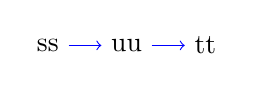
\begin{tikzpicture}
		\node (1) at(0,0) {\Rnode{s}{s}};
		\node (2) at(1,0) {\Rnode{u}{u}};
		\node (3) at(2,0) {\Rnode{t}{t}};
		\draw[->,blue] (1)--(2);
		\draw[->,blue] (2)--(3);
	\end{tikzpicture}
	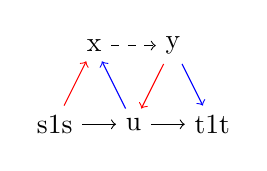
\begin{tikzpicture}
		\node (1) at(0,0) {\Rnode{s1}{s}};
		\node (2) at(1,0) {{u}};
		\node (3) at(2,0) {\Rnode{t1}{t}};
		\node (4) at(0.5,1) {x};
		\node (5) at(1.5,1) {y};
		\draw[->] (1)--(2);
		\draw[->] (2)--(3);
		\draw[->,red] (1)--(4);
		\draw[->,blue] (2)--(4);
		\draw[->,red] (5)--(2);
		\draw[->,blue] (5)--(3);
		\draw[->,dashed] (4)--(5);
	\end{tikzpicture}
\end{figure}
\ncarc[arrows = ->, linewidth=0.5pt, linecolor =red, arcangle = 80, nodesep = 1pt]{s}{u}
\ncarc[arrows = ->, linewidth=0.5pt, linecolor =red, arcangle = -80, nodesep = 1pt]{u}{t}
\ncarc[arrows = ->, linewidth=0.5pt, linecolor =red, arcangle = 80, nodesep = 1pt]{t1}{s1}

Firsly, we could split an edge into a blue one and a red one where $w_r=d_e$ and $w_b=c_e-d_e$. To get a feasible flow, red edges in the new graph should be full.

Since the constraint should be satisfied, we could desgine the third graph above via introducing 2 vertices $x,y$ and an edge $(t,s)$ with weight $+\infty$.
Now we just need to run a max flow algorithm from $y$ to $x$.
Naturally, if the max flow equals $\sum_{e\in E}d_e$, then the constraint is satisfied.

\subsection*{(b)}
Firstly, we need check whether graph $G$ is feasible by algorithm \ref{ex}. This step generate a new graph $H$.

Then we could run Ford-Fulkerson algorithm on $G$ with some refinement:
\begin{itemize}
	\item 
		Source: $s$, sink:  $t$.
	\item
		Initialization:
		\[
			f_{(u,v)}=g_{(u,v)}+d_{(u,v)}
		\] where $g_{(u,v)}$ is the flow at edge $(u,v)$ in graph  $H$.
	\item
		The updating rule becomes:
		\[
			c_f(u,v)=
		    \begin{cases}
			    c_e-f_e & \text{if } (u,v)\in E \\
			    f_e-d_e & \text{if } (v,u)\in E \\
		    \end{cases}
	    \] where $(u,v)=e$.
\end{itemize}
The initialization means that we begin with a feasible way.
And the updating rule ensures every flow is feasible because every edge is positive.
Then like the proof of FF Algo., we could prove that this new algorithm could find a maximum feasible flow with lower bounds.

\section{Misc}
About a day. Dfficulty 3. No collaborator.


\end{document}
